\documentclass[11pt]{article}
\usepackage{deauthor}
\usepackage{times}
\usepackage{graphicx}
\usepackage{xspace}
\usepackage{xcolor}
\usepackage[square,numbers]{natbib}

\newenvironment{denselist}{
    \begin{list}{\small{$\bullet$}}%
    {\setlength{\itemsep}{0ex} \setlength{\topsep}{0ex}
    \setlength{\parsep}{0pt} \setlength{\itemindent}{0pt}
    \setlength{\leftmargin}{1.5em}
    \setlength{\partopsep}{0pt}}}%
    {\end{list}}

\newcommand{\squishlist}{
   \begin{list}{$\bullet$}
    { \setlength{\itemsep}{0pt}
      \setlength{\parsep}{2pt}
      \setlength{\topsep}{0pt}
      \setlength{\partopsep}{0pt}
      \leftmargin=25pt
\rightmargin=0pt
\labelsep=5pt
\labelwidth=10pt
\itemindent=0pt
\listparindent=0pt
\itemsep=\parsep
    }
}
\newcommand{\squishend}{\end{list}}

% use extensively to toggle between paper and TR
\newcommand{\eat}[1]{}
% \newcommand{\papertext}[1]{{\leavevmode\color{blue}{#1}}}
% \newcommand{\techreport}[1]{{\leavevmode\color{red}{#1}}}
\newcommand{\papertext}[1]{#1}
\newcommand{\techreport}[1]{}
\newcommand{\boldpara}[1]{\textbf{\paragraph{#1}}}
% de-facto paragraph format
\newcommand{\stitle}[1]{\par\noindent\textbf{#1}}
\newcommand{\tvcg}[1]{{\leavevmode\color{blue}{#1}}}
\newcommand{\cut}[1]{{\leavevmode\color{lightgray}{#1}}}
\newcommand{\ccut}[1]{} %confirmed cut
\def\plainauthor{Doris Jung-Lin Lee, Aditya Parameswaran}
\def\emptyauthor{} 
\def\plainkeywords{Data visualization, exploratory data analysis, visual querying.}
\def\plaingeneralterms{Documentation, Standardization}

\newcommand{\zv}{\textit{zenvisage}\xspace}
\newcommand{\vida}{\textsc{vida}\xspace}
\newcommand{\sbd}{\textsc{Storyboard}\xspace}
\newcommand{\agp}[1]{\textcolor{green}{Aditya: #1}}
\newcommand{\dor}[1]{\textcolor{blue}{Doris: #1}} 

\newcommand\notes[1]{\textcolor{red}{#1}}

% To make various LaTeX processors do the right thing with page size.
\def\pprw{8.5in}
\def\pprh{11in}
\special{papersize=\pprw,\pprh}
\setlength{\paperwidth}{\pprw}
\setlength{\paperheight}{\pprh}
\setlength{\pdfpagewidth}{\pprw}
\setlength{\pdfpageheight}{\pprh}
%%%%%%%%%%%%%%%%%%%%%%%%%%%%%%%%%%%%%%%%%%%%

\begin{document}
\title{From Search to Recommendation: Towards Visual Discovery Assistant}
% \title{Navigating Visualization Collections}
%\title{Towards a Holistic Workflow for Visual Data Exploration}
\author{\plainauthor\\
\{jlee782,adityagp\}@illinois.edu\\
University of Illinois, Urbana-Champaign}
\maketitle
\begin{abstract}
Visualization is one of the 
most effective and widely-used 
techniques for understanding data. 
Yet, the growing use of visualizations 
for exploratory data analysis 
presses new demands beyond simply 
the graphical presentation 
and visualization authoring 
capabilities offered in existing tools. 
In particular, many data analysis
tasks involve navigating large 
collections of visualizations to make sense
of trends in data;
at present, this navigation is done manually or
programmatically. 
We outline a vision for an
intelligent, interactive, understandable,
and usable tool 
that can help automate
this largely manual navigation: we call our tool \vida\footnote{Vida is short for {\em life} in Spanish.}---short for {VIsual Discovery Assistant}. 
We argue that typical navigation tasks can be 
organized across two dimensions---overall goal 
and precision of specification.
We organize prior work---both our own work, as well
as other ongoing work in this area---across 
these two dimensions, and highlight
new research challenges.
Together, addressing these challenges underlying \vida
can help pave the way for a comprehensive
solution for removing the pain points
in visual data exploration.
% We outline a vision for a new breed of 
% interactive tools that can help automate
% this largely manual navigation process. 
% We argue that these tools need to span two 
% dimensions---precision and task.
% We organize prior work---both our own work, as well
% as other ongoing work in this area---to highlight
% new research challenges
% across these two dimensions.
% Together, addressing these challenges
% can help provide a comprehensive solution 
% for navigating and making sense of 
% large collections of visualizations. 
% In this paper, we describe three areas of visual data exploration facing these challenges. First, we introduce the problem of precise querying: how to search for a desired trend or pattern given the large space of visualizations that could be generate from a given dataset. As vague and complex queries cannot often be addressed through interactions in precise visual querying systems, we introduce a class of intelligent visual querying systems that allows users provide feedback in order to clarify and refine their queries. Finally, even with a omnipotent system that addresses any given visual query, users may not know what to query. Therefore, we advocate for recommendations that facillitates distributional and contextual awareness to help users gain more holistic data understanding, guide them towards meaningful insights, and jumpstart further inquiries. We describe the exemplary systems drawing from both our own work (\zv and \sbd) and ongoing research in the area to highlight future directions and opportunties in this space.
% This paper surveys the emerging field of formally reasoning
% about and optimizing open-ended crowdsourcing, a popular and crucially important, but severely
% understudied class of crowdsourcing—the next frontier in crowdsourced data management. The underlying
% challenges include distilling the right answer when none of the workers agree with each other,
% teasing apart the various perspectives adopted by workers when answering tasks, and effectively selecting
% between the many open-ended operators appropriate for a problem. We describe the approaches that
% we’ve found to be effective for open-ended crowdsourcing, drawing from our experiences in this space.
\end{abstract}

% Eventually, we need to compile all of these into one single file  during submission time. 
%!TEX root = main.tex
\section{Introduction}% 

\par 
With the ever-increasing complexity 
and size of datasets,
there is a growing demand for 
information visualization tools
that can help data scientists make sense of large
volumes of data.
Visualizations help discover 
trends and patterns, 
spot outliers and anomalies, 
and generate or verify hypotheses.
Moreover, 
visualizations are visceral and intuitive: 
they tell us stories about our data; 
they educate, delight, inform, 
enthrall, amaze, and clarify.
This has led to the overwhelming popularity
of point-and-click visualization tools like Tableau~\cite{Stolte2002},
as well as programmatic toolkits like ggplot, D3, Vega, and matplotlib. 
We term these tools as {\em visualization-at-a-time} approaches, since
data scientists need to individually 
generate each visualization (via code or interactions),
and examine them, 
one at a time.


\par
As datasets grow in size and complexity, 
these visualization-at-a-time approaches start to break down,
due to the limited time availability on the 
part of the data scientists---there 
are often too many visualizations to examine for a given 
task, such as identifying outliers, or inferring patterns. 
Even on a single table, 
visualizations can be generated
by varying the subsets of data operated on, 
or the attributes (or combinations
thereof) that can be visualized. 
If we add in various visualization modalities, encodings,
aesthetics, binning methods, and transformations,
this space becomes even larger.


\par
Thus, there is a pressing need for an 
intelligent,
interactive, understandable, usable, and
enjoyable tool that can help 
data scientists navigate
collections of visualizations.
We term our hypothesized tool \vida,
short for {\em VIsual Discovery Assistant}.
Data scientists specify their discovery
goal at a high level,
with \vida 
automatically 
traversing visualizations to provide
solutions or partial solutions for the
specified discovery goal, thereby
eliminating the tedium and wasted
labor of comparable visualization-at-a-time 
approaches.

\par
\stitle{\vida Dimensions.} In order to be a holistic solution for 
navigating collections of visualizations,
\vida must be able to support various discovery
settings. 
We organize these settings along two
dimensions, displayed along the columns and 
rows (respectively) of Table~\ref{fig:table}---first, the overall discovery goal,
and second, the degree of specificity of the goal.
We also cite references (described later on)
for systems that partially provide the necessary
functionality for the given setting.
We call these systems Visual Querying Systems, or VQSs for short.


\begin{wrapfigure}{l}{0.5\textwidth}
\centering
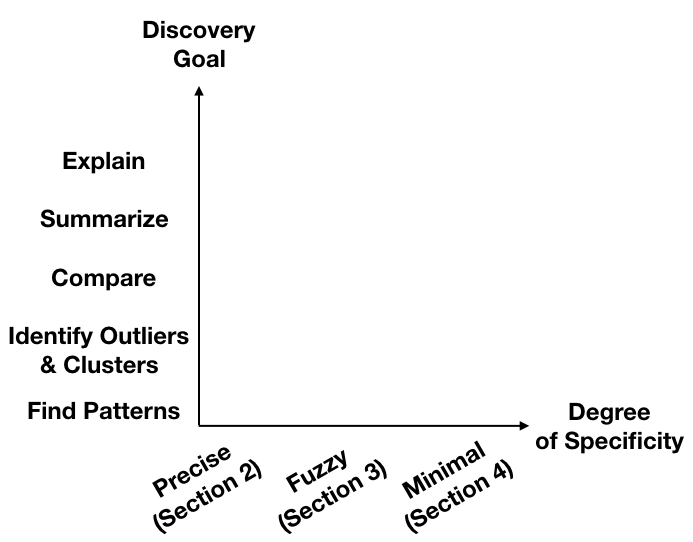
\includegraphics[width=\linewidth]{figures/dimensions_cropped.png}
\vspace{-10pt}
\caption{Dimensions of VQSs. Columns are organized into discovery goals and rows are ordered by decreasing levels of query specificity and correspondingly increasing levels of autonomous assistance.}\label{fig:table}
\vspace{-15pt}
\end{wrapfigure}

\par
 We identify five 
common discovery goals in visual data exploration, organized
along the columns:
{\em finding patterns}, {\em identifying anomalies/clusters}, {\em summarizing}, 
{\em performing comparisons}, {\em providing explanations}.
These five goals borrow borrow from functionalities in existing
systems, as well as related visualization task taxonomies~\cite{Heer2012,Amar2005}.
We omit low-level goals such as filtering or sorting, since
these functionalities are common in 
visualization-at-a-time tools and toolkits.
We also omit goals that go beyond visual data exploration,
such as extrapolation, supervised learning, and cleaning, among others. 

\par 
 We identify three degrees of specificity
for the discovery goal, organized along the rows:
{\em precise}, {\em fuzzy}, {\em underspecified}.
The degree of specificity characterizes the division
of work between how much user has to specify
versus how much the system has to automatically
infer and aid in accomplishing the discovery goal. 
At the topmost row, the onus is placed on the user
to provide an exact and complete specification of 
what the solution to their discovery
goal must look like;
at the middle row, the user can provide
a vague specification of what the solution must look like;
and finally, at the bottom row,
the user provides a minimal specification, or
leaves the characteristics of the solution underspecified,
leaving it up to the system to ``fill in'' the rest.
Naturally, as we proceed down the rows,
it gets harder for the system to automatically
interpret what the user might have in mind as a solution
to their discovery goal.

\begin{table}[!t]
\scriptsize
\centering
\begin{tabular}{l|l|l|l|l|l}
& \multicolumn{5}{c}{Discovery Goals}                                                                     \\ \hline
& Find Patterns & Identify Anomalies and Clusters      & Compare           & Summarize  & Explain          \\ \hline
Precise (Section~\ref{sec:precise}) & \multicolumn{3}{c|}{Zenvisage~\cite{Lee2017}, ZQL~\cite{Siddiqui2016}}                                      &            &                  \\ \hline
Fuzzy (Section~\ref{sec:vague})     & ShapeSearch\cite{Siddiqui2018}   & Scorpion\cite{Wu2013}, Profiler~\cite{Kandel2012}, Natural Language & Natural Language~\cite{Fast2018,Setlur2016,Hoque2017}  &            & Natural Language \\ \hline
Minimal (Section~\ref{sec:minimal}) &               & \multicolumn{1}{c|}{Storyboard~\cite{Lee2018}}      & SeeDB~\cite{Vartak2015}, Storyboard & Storyboard & Storyboard      
\end{tabular}
\caption{Overview of the systems described in this paper. Columns are organized into discovery goals and rows are ordered by decreasing levels of query specificity and correspondingly increasing levels of autonomous assistance.\agp{fix this. add specificity, augment references}}\label{fig:table}
\end{table}




\par
\stitle{\vida Input Modalities.} To support the spectrum of 
demands imposed by the
discovery settings described above, \vida 
must support a range of interactive input modalities,
as displayed in Figure~\ref{fig:vida_architecture},
catering to a range of user expertise and preferences.
These input modalities include 
\squishlist
	\item natural language, via a keyword search box, or a dialog or conversational interface;
	\item interactions, either with an existing visualization, such as brushing-and-linking or hovering, or those that construct a new one, such as drag-and-drop or sketching; and
	\item restricted template queries, involving selection of operations and operands from a drop-down menu.
\squishend
We will provide examples of these input modalities in subsequent sections.
Each of these inputs are compiled down
into a query in a query language, called \vidaql.
Alternatively, expert users may directly invoke \vidaql queries.
\vidaql queries will natively support the five discovery goals,
and will also support combinations thereof, e.g., pattern search followed by 
summarization. 
Another important element is how much does a user actively ``request'' (pull)
versus \vida ``recommending'' visualizations (push). 
Given that we expect \vida to support a range of specificities,
\vida must support both push and pull, with pull decreasing
in importance, and push rising in importance, as we go from precise to minimal.

\begin{wrapfigure}{r}{0.5\textwidth}
\centering
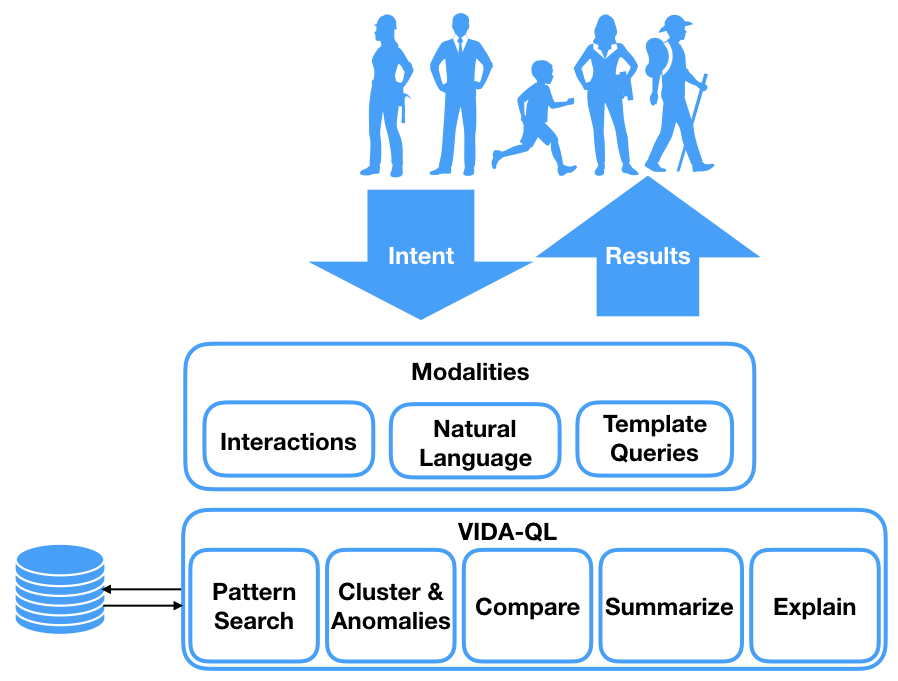
\includegraphics[width=\linewidth]{figures/VIDA_architecture.png}
\vspace{-10pt}
\caption{\vida Architecture\label{fig:vida_architecture}
\vspace{-15pt}
}
\end{wrapfigure}

% \begin{wrapfigure}{r}{0.5\textwidth}
%   \begin{center}
%     \includegraphics[width=0.48\textwidth]{birds}
%   \end{center}
%   \caption{Birds}
% \end{wrapfigure}



% Common framework and module means there are underlying functionalities can be shared (e.g. statistical modules, data heavy-lifting operations)
% - From the top: many different types of users (novices/experts), each with some high-level intent in one of the following modalities:
%      - Interaction: produces as an output either through the creation a visualization (e.g. sketching, drag-and-drop) or changes upon a visualization (e.g. brushing, selections, clicks)
%      - Partial specification includes some minimal input such as input X,Y of interest
%      - Either that or user can directly specify their query exactly in VIDA-QL
% - VIDA-QL contains 5 discovery modules which each have their own "push and pull" components, i.e. work with both search and recommend.

\par
\stitle{Outline.}
The rest of our paper is organized along the degree of specificity
of discovery goal, and we will allude to the specific discovery
goals as well as input modalities as we go along. 
The degree of specificity of the discovery goal is the factor
that most significantly affects the architecture of \vida,
with the complexity increasing as the specificity decreases. 

\par We begin by discussing the 
the {\em precise} setting (Section~\ref{sec:precise}).
We describe \zv~\cite{Siddiqui2016} 
as an example of a solution for
this setting, and thereby a starting point for \vida,
partially eliminating the problem
of having to manually examine large numbers 
of visualizations for a given discovery goal, 
which can be error-prone and inefficient.


\par However, a design study using \zv demonstrates
that the precise setting is insufficient for
addressing all of the demands of real-world use-cases~\cite{Lee2017}.
In particular, users do not have
a clear understanding of their intent or specification 
without looking
at example visualizations or summaries of the data,
and at the same time, their intent or specification is
often not expressible clearly, requiring 
vague or fuzzy high-level notions.

To bridge the gap between the user's high-level
intent and the system demands,
we outline a set of research challenges
that goes beyond simple precise visual querying, by
(a) supporting a wider class of vague or ``high-level''
queries, thereby increasing the expressiveness
of \vida (Section~\ref{sec:vague});
and 
(b) making it easier to know what to query
by recommending visualizations that provide
a high-level understanding of the data (Section~\ref{sec:minimal}).

\agp{We should clarify somewhere that most of our concern is going to 
be the interfaces or query languages, as opposed to optimization,
leveraging parallelism, MQO, sampling, pruning,
which has seen some work --- ZQL, SeeDB, ...}

% In addition, we find that users often do not have a good idea of what they want to query for without looking at example visualizations or summaries of the data. To bridge the gap between user's high-level intent and what the system operates as inputs, we advocate that future research needs to look beyond simple precise visual querying by : 1) making visual query system more expressive by supporting a wider class of vague queries (Section~\ref{sec:vague}) and 2) making it easier to know what to query by recommending visualizations that facilitate data awareness (Section~\ref{sec:minimal}).
% \par Accordingly, the next row in the table highlights a growing class of \textit{intelligent visual querying system} (IVQS) that interprets the `vagueness' of queries and allow users to tweak or refine their queries through a feedback mechanism. \dor{I think we need to expand this definition depending on the new content that we will be adding, ShapeSearch, SeeDB, Scorpion?} 
% \par To address the problem of guiding users to portions of the data that they might be interested in querying, Section~\ref{sec:minimal} introduces systems that help users become more aware of their dataset and visualize where they are in their analysis workflow. The challenge in building these systems involves understanding what types of visualizations should be recommended to facilitate data awareness. As an example, we describe our work on \sbd, a system that provides data summaries and guides users through informative subsets of data. Finally, we discuss related works on how visualizing provenance and situational information can guide users towards more informative analysis actions.
%!TEX root = main.tex
\section{Precise Visual Querying\label{sec:precise}}
Visual analysis often reveal important anomalies or trends in the data\cite{Morton2014}. However, it is often challenging to find the appropriate piece of information to realize these insights.

\subsection{Motivating Example}
Astronomers from the The Dark Energy Survey (DES)\cite{Drlica-Wagner2017} are interested in finding anomalous time series to discover astrophysical transients (objects whose brightness changes dramatically as a function of time), such as supernova explosions or quasars. When trying to find celestial objects corresponding to supernovae, which have a specific pattern of brightness over time, scientists need to individually inspect the visualizations of each object until they find ones that match the pattern. With more than 400 million objects in their catalog, each having their own set of time series brightness measurement, the process of manually exploring a large number of visualizations is not only error-prone, but also overwhelming for scientists who do not have extensive knowledge about their dataset.  
% Intention driven task-based querying (Precise search)
\par The astronomy use case highlights a common challenge in exploratory data analysis (EDA). There is often a large space of possible visualizations that could be generated from a given dataset and manual search through this large collection is inefficient. Visualization authoring tools such as Tableau and Excel focusses on presenting one visualization at a time. There is no systematic way to create, compare, and query large collections of visualizations. 
%\par There has been many related work in this space varying different dimensions of possible visualizations, including visual encodings~\cite{showme}, data facets, . We will focus on  
\subsection{Effortless Data Exploration with \zv}
\par The challenges presented earlier points to a need for tools that enables users to create and search through large collections of visualizations. Therefore, we developed \zv a visual query system that allowed users to search through large collections of visualizations. \zv is built on top of a querying language called ZQL, which provides a mechanism for managing collections of visualizations\cite{Siddiqui}. Contrary prior work on visualization languages for specifying visual encodings of individual visualizations~\cite{Stolte2002,Wilkinson2005}, ZQL supports high-level queries over visualization collections, such as composing, sorting, filtering a collection of visualization. ZQL functionals and primitives can be constructed into rich and expressive query semantics, with functionalties including : 
\begin{itemize}
	\item Finding top-k visualizations whose y values are most or least similar from a queried visualization (e.g. Find other cities with sold price over time similar to Manhattan. Varying along \textsc{city} while keeping \textsc{x=time,y=AVG(price)} fixed.) 
	\item Comparing across a collection of visualizations by iterating over one or more x, y, z attributes while fixing other attributes (e.g. Find a y attribute that varies with time similarly how average price changes over time)
	\item Finding a pair of X and Y axes where two specific visualization instances differ the most. (e.g. For what pair of attributes does the products `stapler' and `chair' differ the most?)
\end{itemize}
\par Given a ZQL query, \zv parses the query into a graph of visual component nodes(containing visualization information, such as X, Y columns) and task nodes (common and user-defined primitives for processing visual components, such as sort-filter). \zv then performs query optimization to merge together multiple nodes, as well as reducing the processing time required for individual visualization components. Using the optimized query plan, the executor compiles visual nodes into SQL queries for retreiving the visualization data and postprocesses the result via the defined operations. 
\par While ZQL provides powerful mechanism for expressively specifying queries on large collections visualizations, writing ZQL queries can be daunting for novice users. Therefore, we extracted a typical workflow of visualization querying (finding top-k most similar visualization from a collection with fixed X,Y while varying Z) to allow users to formulate ZQL queries through interactions. The user can either directly input ZQL queries through a frontend table input or their frontend interactions is mapped into ZQL queries. The query results are rendered as a ranked list of visualizations in the Results panel in the frontend. \zv is a full-fledged visual querying system that supports a variety of querying interactions as illustrated in Figure~\ref{fig:modalities}. In the following section, we will discuss the design process of how we developed this visual query system and the lessons that we have learned for designing future visual data exploration systems.

\begin{figure}[h!]
\label{fig:modalities}
\centering
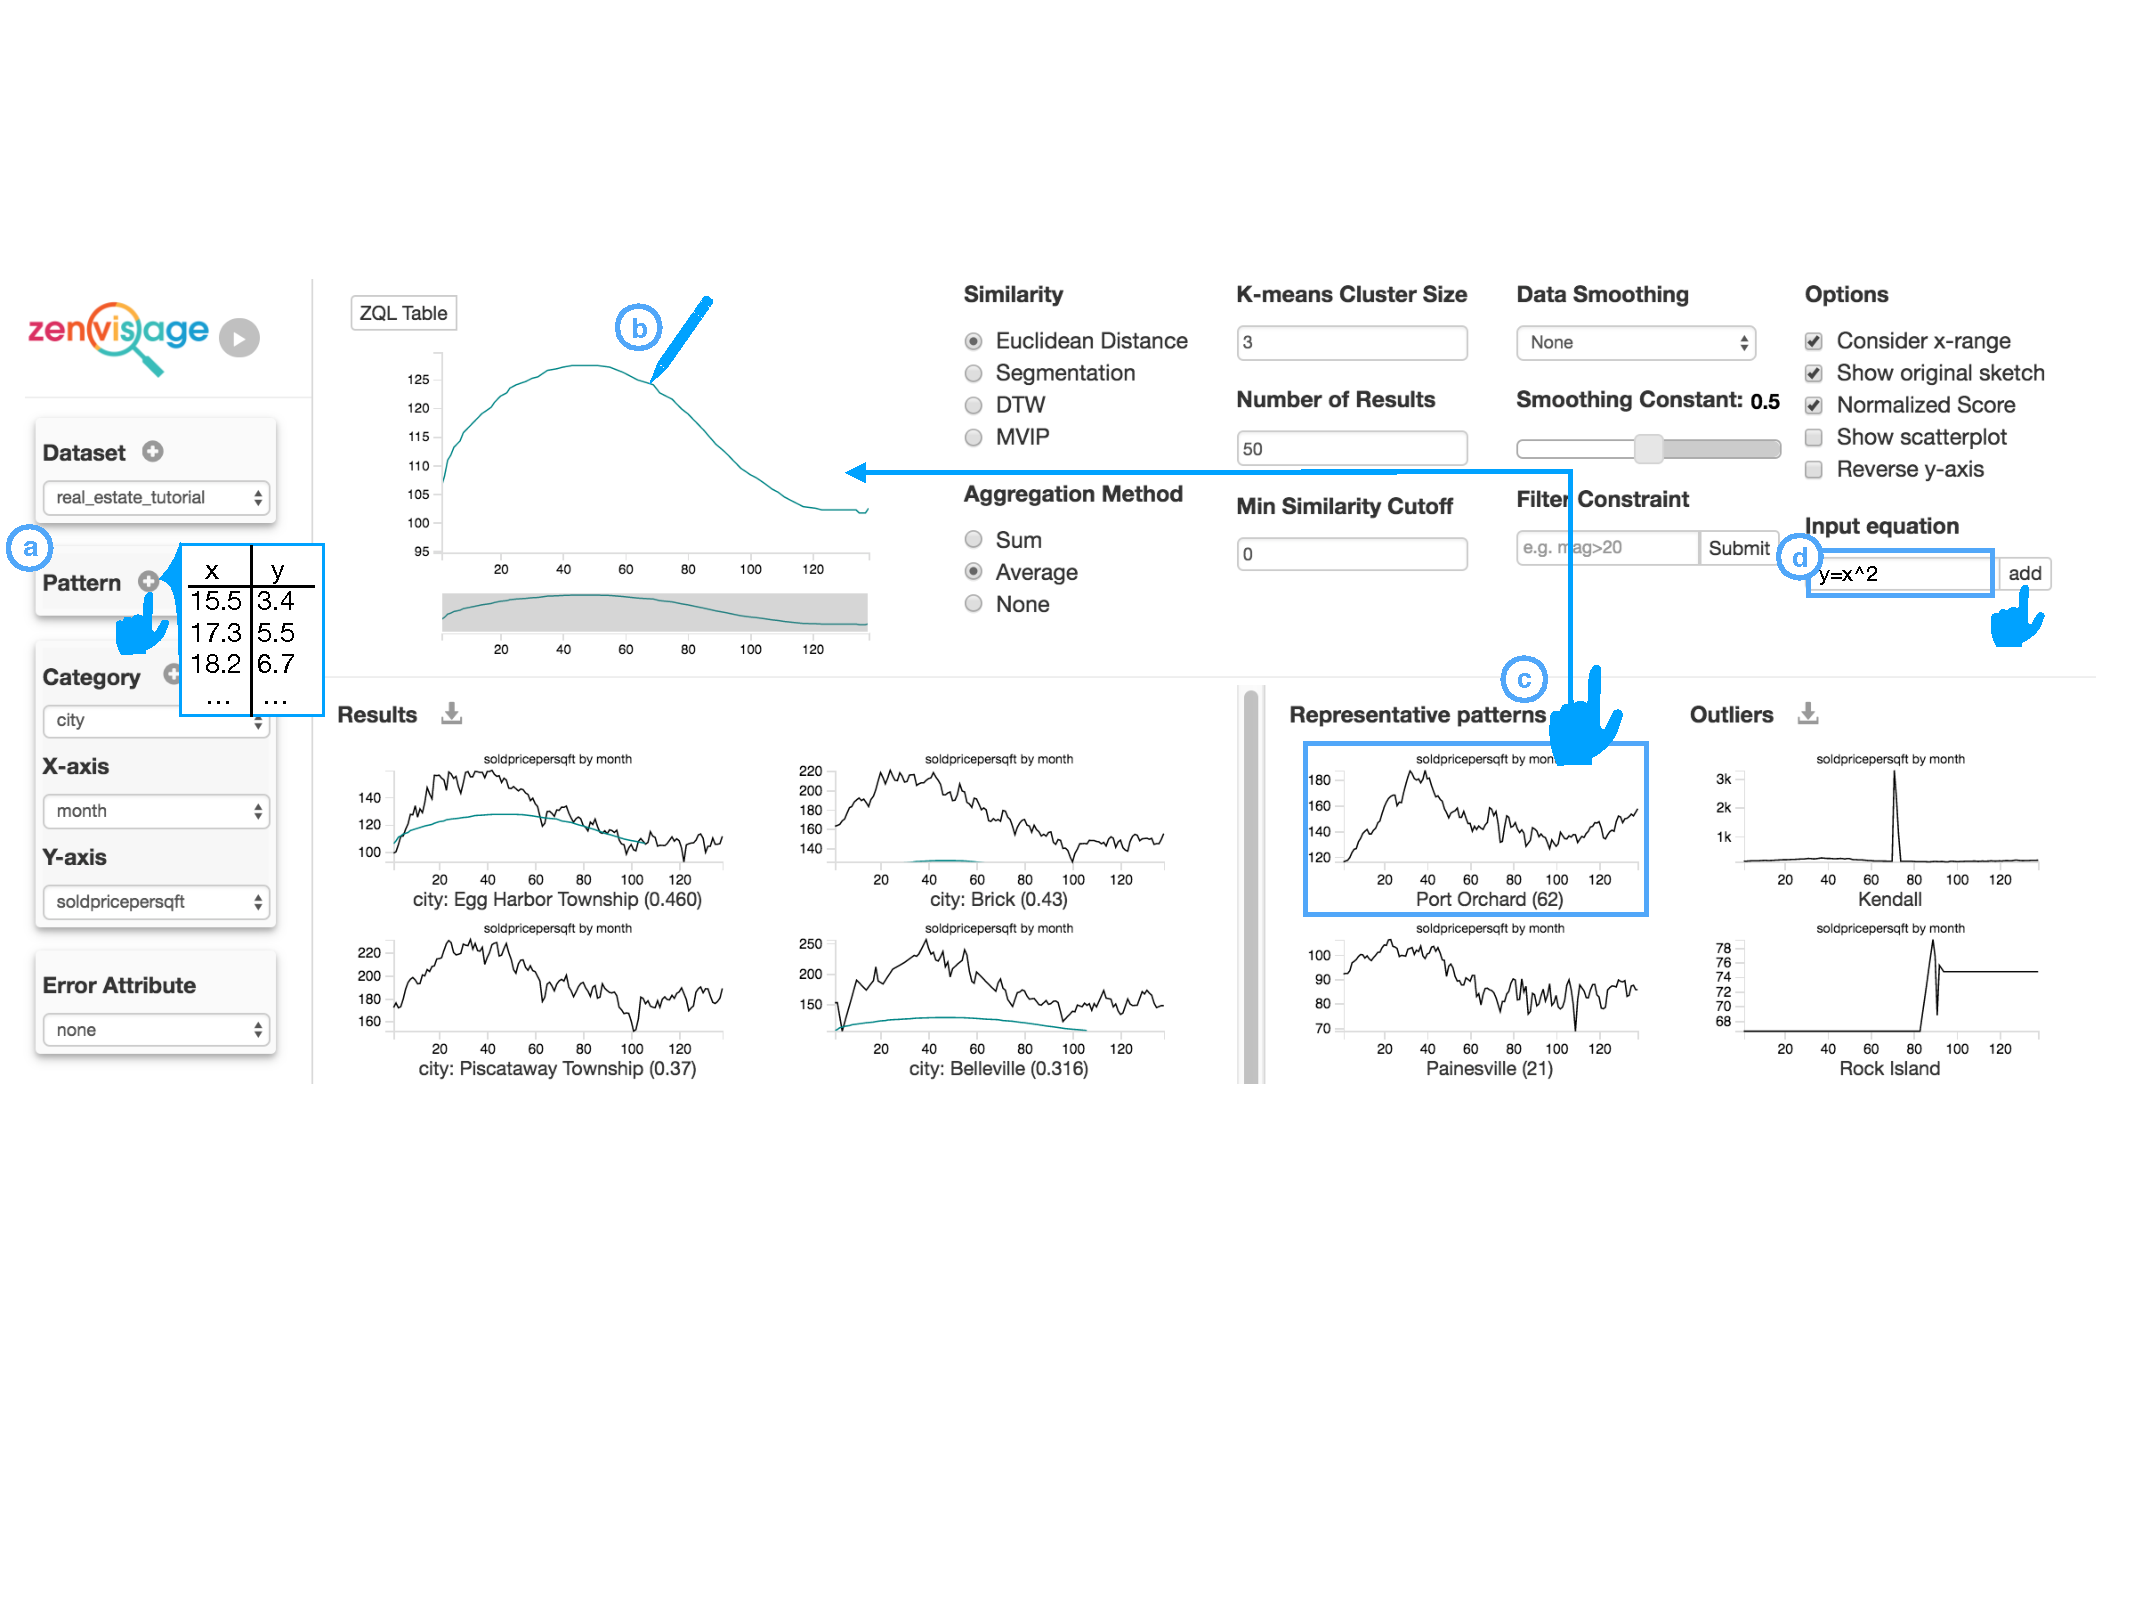
\includegraphics[width=0.8\textwidth]{figures/modalities.pdf}
\caption{\zv offers a variety of querying modalities, including: a) uploading a sample pattern from an external dataset as a query, b) sketching a query pattern, c) dragging-and-dropping an existing pattern from the dataset, and d) inputting an equation as a query.}
\end{figure}

%!TEX root = main.tex
\section{Hypothesis Formation and the cycle of visual analysis\label{sec:hypothesis}}
\subsection{Visual Querying in the \textit{Sensemaking Framework}}
\zv is an example of a \emph{precise visual querying system (PVQS)}, which accepts precise queries as an input, expressed through interactions or directly specified via the querying language. In developing \zv, we collaborated with scientists from astronomy, genetics, and material science in a year-long participatory design process~\cite{Lee2017}. In particular, we study how various features impacts analyst's ability to rapidly generate new hypothesis and insights and perform visual querying and analysis. Our findings offered design guidelines for improving the usability and adoption of next-generation VQSs. More importantly, in this section, we focus on applying our findings on visual querying to the context of supporting the full cycle of visual data exploration. 
\begin{figure}[h!]
\label{fig:cycle}
\centering
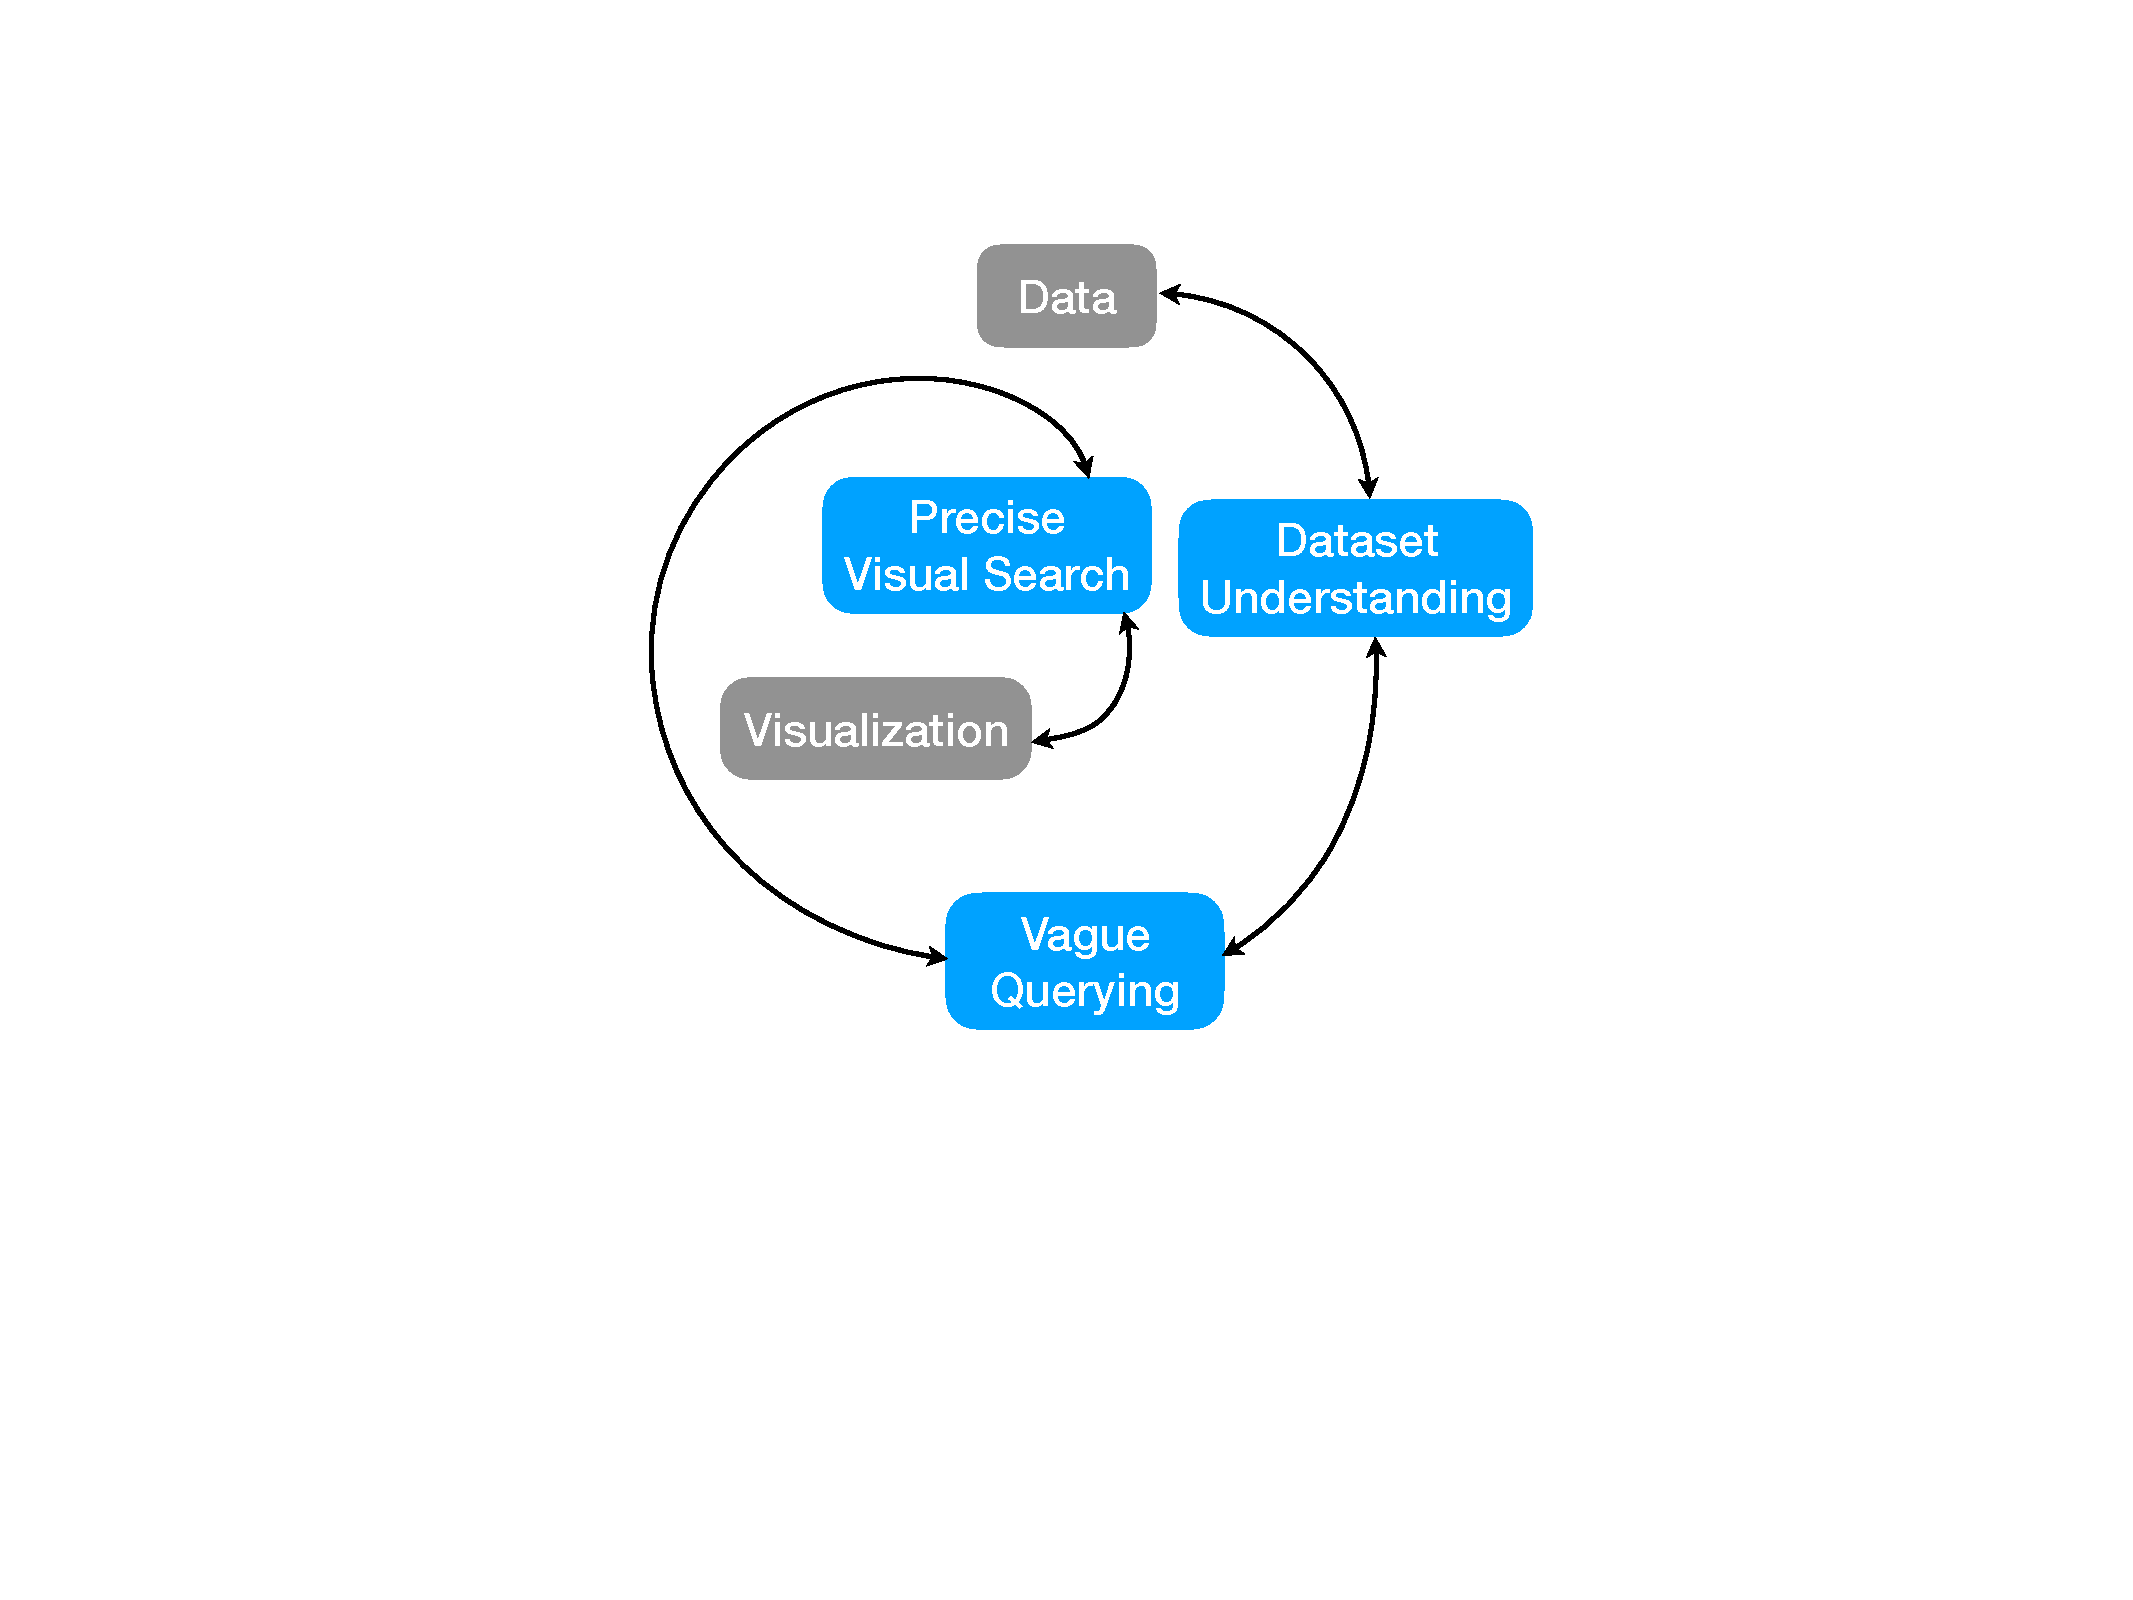
\includegraphics[width=0.5\linewidth]{figures/cycle.pdf}
\caption{Cycle of visual data exploration.}
\end{figure}
%We highlight two of the key findings related to this goal below.: Our participatory design findings points towards future ----- in supporting a cycle of ---.  ----advocate ---cycle of visual analysis. 
% \begin{itemize}
% 	\item Essential ingredient in facilitating intelligent vague querying and exploration.
% 	\item This is a human process (\cite{Heer2012,Pirolli})
% 	\item Iterative Hypothesis Exploration/Refinement : argue that the following properties is important to sustain this “cycle of visual analysis” 
% \end{itemize}
\stitle{The Need for Supporting Complex Vague Expressive Querying}
\par When users are querying with a PVQS, they often need to translate their ambiguous, high-level questions into an plan that consists of multiple interactions to incrementally address their desired query. Participants in our \zv design study often created unexpected workflows that chain together multiple analysis steps, including interactions, controls, and queries in order to address a higher-level research question. For example, the geneticists in our study repeatedly explored representative trends to gain an overall sense of what typical profiles exist in the dataset and queried mainly through drag-and-drop of these representative trends. Variations to their main workflow also include changing cluster sizes and display settings to offer them different perspectives on the dataset and filtering on data attributes. 
\par The expressiveness of PVQSs comes from the multiplicative effect of stringing together combinations of interaction sequeneces into a customized workflow. Designing features that diversifies potential variations and helps the creation of multiple analysis workflows expands the space of actions that could be performed during the analysis. 
\par However, even with many supported interaction, there were still complex multi-step queries that could not be expressed through this framework. One example is the use of vague descriptors for matching to specific data characteristics, such as find me light curves that are flat and `without noise', or patterns that `exhibits irregularities'. While we could ---- in ZQL, 
One solution is to divert to ZQL. 
\par There is an inevitable design trade-off between the query expressivity and interface usability\cite{Morton2014,Jagadish2007}. Balance between language/querying complexity versus expressiveness. The extensibility of these systems or querying language also comes with the cost of potentially overloading the users with too many potential options to chose from. In Section~\ref{sec:vague}, we survey related work in this area and advocate for ----- vague querying. More importantly pointed towards a need for vague querying. Give some examples of vague querying.
%The main workflow for the astronomers in our user study involves \textit{enriching}, either through the creation of groups or via filtering data subsets. The main workflow for material scientists involves \textit{exploiting}, since they spend the majority of their efforts performing ``close-reading'' of individual visualizations to understand the relationships between  physical variables. 
\stitle{Top-down and Bottom-up Querying Modalities}
\par We employed Pirolli and Card's~\cite{Pirolli} information foraging framework for domain-experts to contextualize our study results. Pirolli and Card's notional model distinguishes between information processing tasks that are \textit{top-down} (from theory to data) and \textit{bottom-up} (from data to theory). In the context of visual querying, users employ top-down approaches by starting with a hypothesis on what patterns to look for and express it through sketching or inputting an equation (Figure~\ref{fig:modalities}b,d). On the other hand, bottom-up approaches originate from the data (or equivalently, the visualization). For example, the user may drag and drop a visualization of interest in the dataset as the input query or upload a visualization from an external dataset (Figure~\ref{fig:modalities}a,c). 
\par Our interactions with the scientists showed that \emph{bottom-up querying via drag-and-drop was more intuitive and more commonly used than top-down querying methods when the users have no desired patterns in mind}, which is commonly the case for exploratory data analysis. One of the main reason why participants did not find sketching useful was that they often do not start their analysis with a pattern in mind. Later, their intuition about what to query is derived from other visualizations that they see in the VQS, in which case it made more sense to query using those visualizations as examples directly. Similarly, while functional fitting is a common operation in scientific data analysis, querying by equation is also unpopular, since it is challenging to formulate functional forms in an prescriptive, ad-hoc manner without seeing what the common patterns in the dataset are. 
\par While the usage of each querying feature may vary from one participant to the next, a key design principle that came from this finding was the need for visual query systems to provide visualization recommendations that can help analysts jumpstart their exploration. We found that many users made use of the representative trends and outliers visualizations provided by \zv as contextual information to better understand their data (e.g. after a filter is applied) or to query based on these recommended visualizations (e.g. find visualizations that are similar to the one in the largest representative clusters). 
\par As evident from the representative and outliers in \zv, recommendations facillitate smoother flow of analysis by closing the loop between the two modalities of querying and exploration, thus ensuring that user is never stuck or out of ideas at any point during the analysis. Typically, visualization recommendation systems seeks to accelerate the process of discovering interesting aspects of the data by broadening exploration during exploratory analysis. In Section~\ref{sec:understanding}, we advocate recommendation systems should not only focus on data discoverability aspect of exploration, but also contribute towards helping users gain a better awareness and understanding of the context of their analysis and scope of their data.

%for the importance of building recommenders provides that contributes towards data awareness and understanding but also -----. One ----- it does this by going towards better data understanding.
%. an accurate understanding of the context of analysis and scope of data.  but also contribute towards ---- data understanding.
%thought of through the notion of data discoverability ----understanding and finding unseen data. 
% \subsection{Challenges Ahead}
% The goal here is to help novice submit precise queries without SQL background, easy to use interface. Our study found that VQS does more than just this, but still not enough.
% \begin{itemize}
% 	\item Precise Search Fail to understand intricacies of user need/intent, need more expressivity/flexibility for querying.
% 	\item  No perfect training workload, real-world data + task is noisy and complex. 
% 	\item towards more holistic model for insight discovery
% \end{itemize}

%!TEX root = main.tex
\section{Vague Intelligent Search\label{sec:vague}}
Accounting for user interaction, mental models. More global objective taking into account user with the goal of dataset understanding rather than task completion.
\subsection{Challenges}
\begin{itemize}
\item Inferring user intent in querying and context is important (both in terms of user input and what is recommended)
\item tools can not assume user has querying intention. exploration without intention, user don’t know what they are searching for --> Recommendation.
\item The important thing here is identifying what should be done by the system v.s. requested from user. Inappropriate choice of these will result in lack of expressibility and user feeling lack of control of analysis, limiting exploration.
\item Need for a unified framework of inference to take all of these into account (e.g. natural language, etc)
\end{itemize}
\subsection{\sbd: Navigating Through Data Slices with Hierarchical Summary of Visualizations}
%!TEX root = main.tex
\section{Towards Dataset Understanding\label{sec:understanding}}
One of the key goals of visual data exploration is to promote a better understanding of the dataset that enables users to make actionable decisions. While our focus in the previous sections have focussed on intention-driven queries, where users have some knowleldge of what types of questions he may be interested in. This section discusses general query-free recommendations and continual provenance that helps users become more aware of the dataset with respect where they are in their analysis workflow. 
\par Situations where there is an absence of explicit signals from the user can happen in two scenarios: 1) user is at the beginning of their analysis (commonly known as the `cold-start' problem) and 2) user doesn't know what to query for, which is the situation derived from our \zv finding in Section~\ref{sec:hypothesis}. In this section, we will describe \sbd, a system that provides data summaries and guides users through infromative subsets of data, as an example of ------. Then, we will discuss three different types of data understanding and awareness during visual data exploration and highlight the challenges ahead and opportunities for these notions of data understanding.
\subsection{\sbd: Navigating Through Data Slices with Hierarchical Summary of Visualizations}
%understanding distributions (distribution awareness)
%introduce problem + challenge
\par Common analytics tasks, such as causal inference, feature selection, and outlier detection requires studying the distributions or patterns at different levels of data granularity~\cite{Anand2015,Wu2013,Heer2012}. However, without knowing \textit{what} subset of data contains an insightful distribution, manually exploring distributions from all possible data subsets can be tedious and inefficient~\cite{Sarawagi1998,Sarawagi2000}. In order to explore different data subsets, a user would first have to construct a large number of visualizations corresponding to all possible data subsets, and then, navigating through this large space of visualizations to draw meaningful insights. The lack of a systematic way to perform these excercises makes the
%there is no systematic way to perform these exercises.
% explain what storyboard does
\par To this end, we present \sbd, an interactive visualization summarization system that automatically selects a set of visualizations to summarize the distributions within a dataset in an informative manner. Figure~\ref{sbd} illustrates an example dashboard generated by \sbd from the Police Stop Dataset \cite{police}, which contains records of police stops that resulted in a warning, ticket, or an arrest. The attributes in the dataset include driver gender, age, race, and the stop time of day, whether a search was conducted, and whether contraband was found. We requested \sbd to generate a dashboard of 9 bar chart visualizations with x-axis as the stop outcome (whether the police stop resulted in a ticket, warning, or arrest/summons) and y-axis as the percentage of police stops that led to this outcome. First, at the top of our dashboard, \sbd highlights three key data subsets that results in a high arrest rate, which looks very different trend than the overall (where the majority of stops results in tickets). Following along the leftmost branch, we learn that even though in general when a search is conducted, the arrest rate is almost as high as ticketing rate, when we look at the asian population, whether a search is conducted had less influence on the arrest rate and the trend resembles more like the overall distribution.
\begin{figure}[h!]
\label{fig:sbd}
\centering
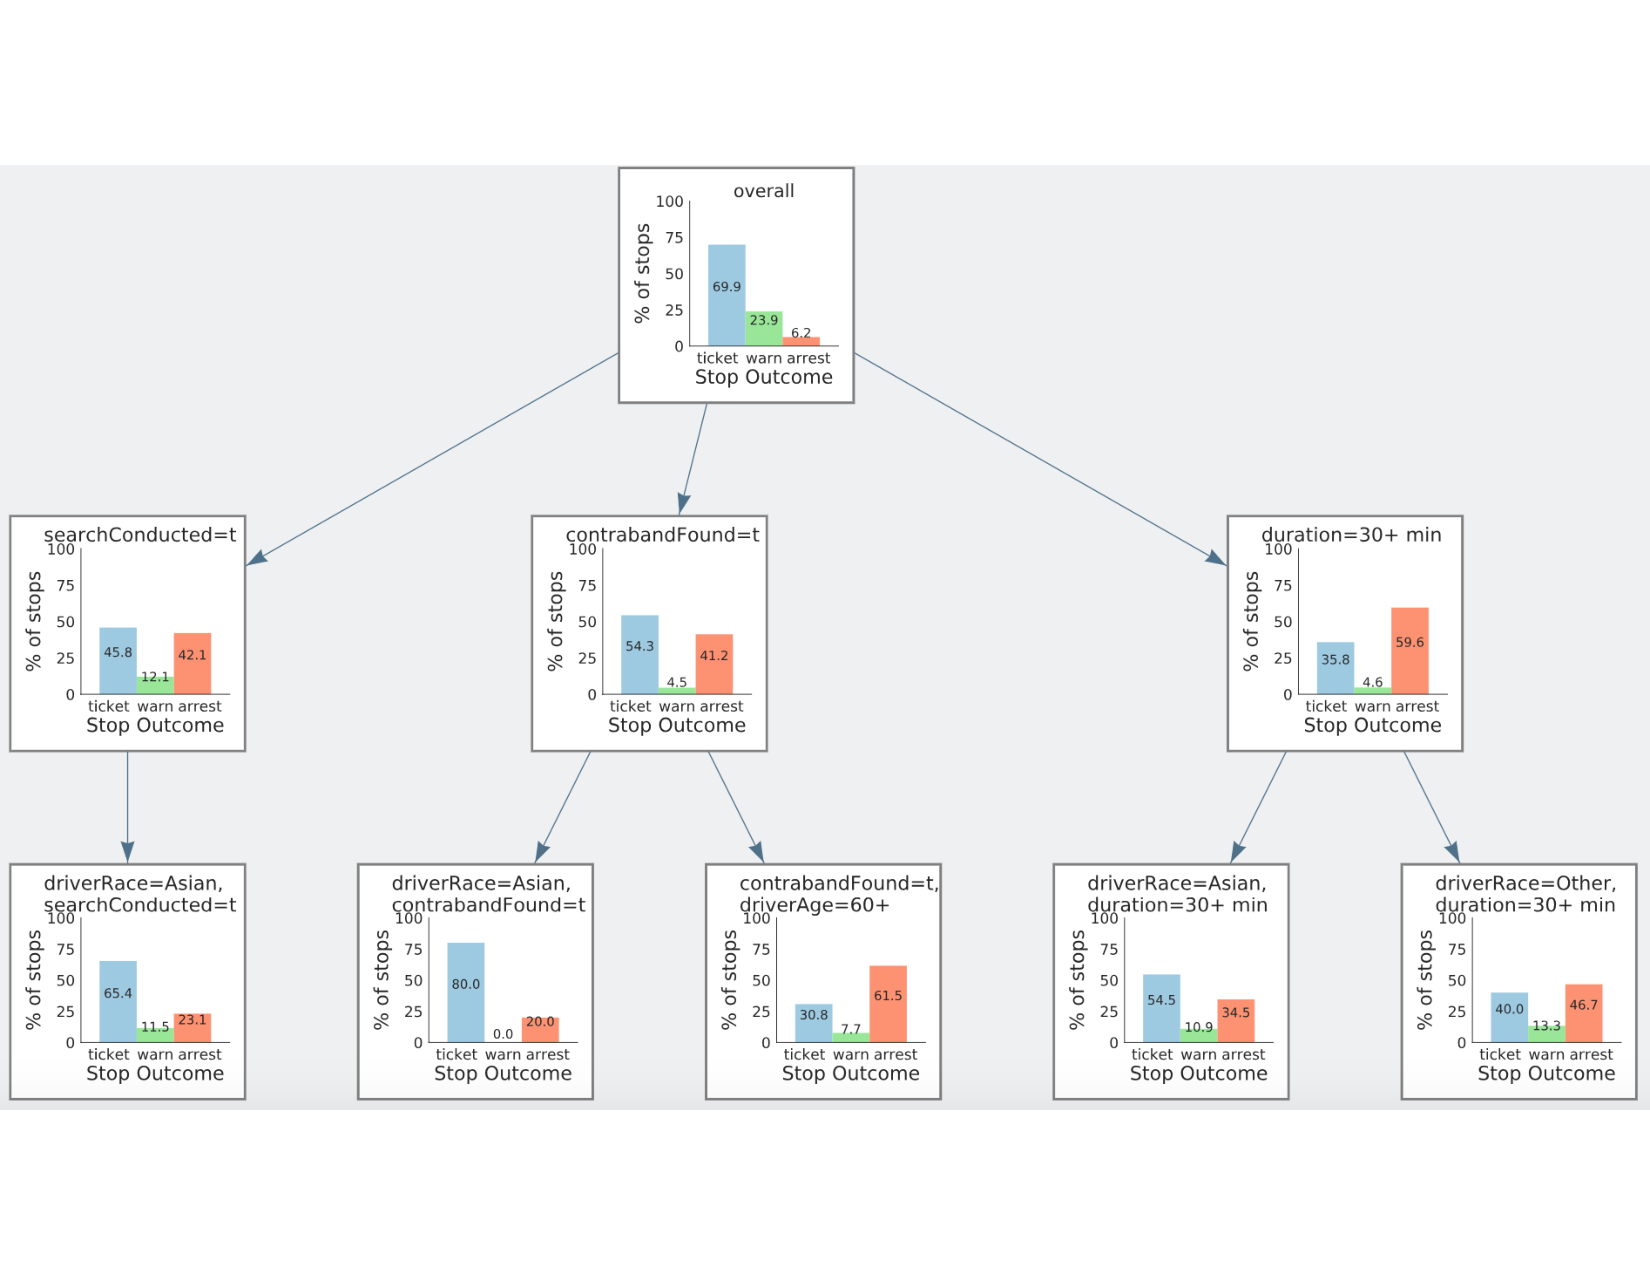
\includegraphics[width=0.7\linewidth]{figures/storyboard.pdf}
\caption{Example dashboard generated by \sbd summarizing the key insights in the Police dataset.}
\end{figure} 
% one paragraph on motivation on objectives and explain lattice + traversal 
\par While such summary dashboards are useful for making sense of relationships between data subsets, finding effective visualizations to summarize a dataset is not as trivial as picking individual visualizations that maximizes some statistical measure, such as deviation~\cite{Vartak2015}, coverage~\cite{Sarvghad2017}, or significance testing~\cite{Anand2015}, which can often result in misleading summarizations. The key insights of our work is 


For example, our insight regarding 

The above example demonstrates a scenario where the selection of an improper reference (female) for comparing the visualization (black female) against results in misleading insights. In \sbd, we formulate an objective where a visualization is \emph{actually} interesting when it deviates from and can not be explained by \emph{even} its most informative reference.

%explain distribution awareness + its application, its relationship with dataset understnading + how it can be used in other contexts.
\par Our user study evaluations show that \sbd guides users to make better predictions regarding unseen visualizations, ranking attribute importance, and retreival of interesting visualizations compared to the baselines. The effectiveness of \sbd largely comes from how it helps analysts become more \emph{distributionally aware} of the dataset. We define \emph{distribution awareness} as the aspect of data understanding in which analysts make sense of the key distributions across different data subsets and their relationship in the context of the dataset. Even though it may be infeasible to examine all possible data subsets, with distribution awareness, the analyst will still be able to draw meaningful insights and establish correlations about related visualizations by generalizing their understanding to make predictions regarding the unseen visualizations. 

How ----- is underexplored 
future research 
building systems that ---

%building future systems that effectively guide analysts towards more meaningful stories for further investigation.

\subsection{Challenges Ahead}
\par Distribution awareness highlights one example of data understanding that -----. In this section, we will discuss several other types of data understanding that is essential for effective visual data exploration. Recommendation providing better understanding for overall dataset and understanding. 
While the notion of distribution awareness is useful when we are looking at user understanding at a static point in time in the analysis (e.g. during cold start), we introduce two complementary notions of data understanding (contextual and situational awareness) when considering dynamic visual exploration in the context of an analytic workflow.
	
\stitle{Contextual awareness} serves to ---- in a dynamic exploration situation, keep track of what filter is in play, what dataset/ schema am I looking at, which operations have been applied to the data that I'm looking at? Related to provenance for the current time. 
Within a dataset, structure and provenance is essential to help users navigate and provide users with sense of coverage and completion. This is an important but underexplored area. (viz-sum, Sarvghad et al 2017)
Mechanisms that provides distribution awareness can effectively couple with contextual awareness in a dynamic exploration situation. For example, the representative and outlier patterns in \zv provides summaries of the current context of the data. When a dataset is filtered, the representative trends are updated accordingly. By understanding both the context (i.e. I'm only looking at data filtered with ....), the distribution awareness learn things on the context, provides
an overview of typical trends for the data to be queried. better understanding of what's in the dataset that I'm looking at. 
\stitle{Situational awarenss}: 
related to provenance, as a function of time.
- provenance of schema and attribute understanding (coverage, etc) . Similar to situational awareness (cite Tory)


\par Note that while the discussion above have been focussed on how to design systems that can help facillatate these aspects of user's awareness in dataset understanding, these ideas can be generalized to principles in deisinging the types of intelligent querying systems discussed in Section~\ref{sec:vague}. An intelligent visual exploration system needs to be distributionally, contextually and situationally aware, by make use of information about the data (distribution awareness), the analytic context, and situation jointly in making timely recommendations. For example, contextual awareness can inform the system that the user's current ---- x,y, main visualization, while a distributionally aware system may recommend a highly-skewed data subset as interesting, a sitational aware system may realize a variable have been explored extensively in the past and recommends it accordingly. In other words, these intelligent visual query system not only needs to facillatate these aspects of data understanding, but also need to make use of this information to make inference and recommendations in an interpretable manner that can guide analysts towards meaningful stories and insights for further investigation.

inference and descisions intepretable.

, rather than the system's awareness of the user's context, situation ,etc. Ideally, an intelligent system  should 


related works have focussed on making specification easier, but not really trying to understnad user intent or what might the user want to see.

%!TEX root = main.tex
\section{Concluding Remarks\label{sec:conclusion}}

% Data is agnostic to the user, intention ---, by building tools---, Section \ref{sec:precise} to \ref{sec:vague} have focussed on extracting what user want from data. bridging together what user want from data, what data has to offer, supporting interactive discourse between the two. 
%  Either using one-size-fits-all statistics, templates, heuristics as a solution or problem only applicable to a subset of analytic tasks\cite{Vartak2015,Vartak2017}. 

In this paper, we advocate supporting a desiderata consisting of  3`I's in the cycle of visual data exploration:
\begin{itemize}
	\item \textbf{Informative}: Section~\ref{sec:precise} discusses how precise visual query systems provide informative visualizations to accelerate the process of data discovery. 
	\item \textbf{Interactive and iterative}: Section~\ref{sec:vague}
	Joining the flow, query refinement, dialogue (not a one-shot query), feedback and recommendation, expressivity (how easy is it to express what to do via interactions) and diversity of actions that could be performed.
	\item \textbf{Integrated}: Section \ref{sec:understanding} discusses the challenges and opportunities in moving from intention-driven querying to facilitating more integrated data understanding and awareness during the analysis workflow.
\end{itemize}
\section*{Acknowledgement}
A. P. acknowledges support from grants IIS-1513407 and IIS-1633755 awarded by the National Science Foundation, grant 1U54GM114838 awarded by NIGMS and 3U54EB020406-02S1 awarded by NIBIB through funds provided by the trans-NIH Big Data to Knowledge (BD2K) initiative (www.bd2k.nih.gov), and funds from Adobe, Google, and the Siebel Energy Institute. The content is solely the responsibility of the
authors and does not necessarily represent the official views of the funding agencies and organizations. \dor{copied this from the crowdsourcing vision paper, might have to change grant number and sources accrodingly. Might also want to include acknowledgement for collaborators here too.}
{\footnotesize \bibliographystyle{named}
\bibliography{reference}}
\end{document}
